\section{Introduction}
\label{sec:introduction}

\par The main objective of this laboratory assignment is to study the following circuit. For that we will be using two methods that we learnt in TCFE class: the Mesh Method and the Node Voltage Method. Then, we want to see if the values that we obtain in this two methods are the same and if they are equal to the ones of Ngspice. We decided to separate this work in other three sections. In the first one,Analysis, we will explain the theoretical analysis of this circuit, the methods that we used to analyse it  and the theoretical values of current and voltage, for that we use the math tools of Octave. Using Ngspice tools, in the second section Simulation, we will present a simulation of our circuit and compare it with the previous theoretical results. Lastly, Conclusion, we will summarise the contents of the report and discuss the achieved results.

\begin{figure}[h] \centering
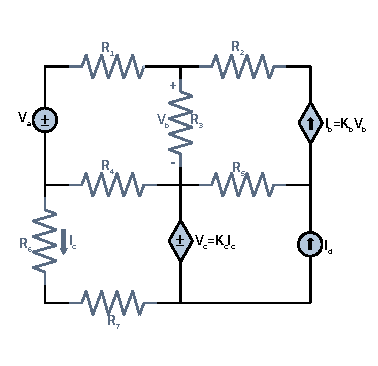
\includegraphics[width=0.8\linewidth]{Circuit.pdf}
\caption{Circuit}
\label{fig:circuit}
\end{figure}
